\documentclass[12pt, letterpaper]{article}
\usepackage[utf8]{inputenc}

\usepackage{geometry}
\geometry{a4paper, total={6in,10in}}

\usepackage{palatino}
\fontfamily{ppl}\selectfont

\usepackage{graphicx}
\graphicspath{{images/}}

\usepackage{csquotes}

\usepackage{tikz}

\title{\textbf{\Huge Introduction to SETS}}
\author{Aviral Janveja}
\date{}


\begin{document}

\maketitle

The concept of \textbf{Set} serves as a fundamental part of present day mathematics.\\ 
Today, the knowledge of sets is required to study almost every branch of mathematics from relations \& functions to geometry and probability.

\section{What is a Set ?}
\begin{displayquote}
\textbf{Definition : A set is a well-defined collection of elements.}
\end{displayquote}
\textbf{For example},\\ 
``The set of alphabets in the english language" is a well defined collection. However, something like ``the five best mathematicians of the world" is not a well defined collection.\\
Sets are usually denoted by capital letters $A, B, C$ and so on. The elements of a set are usually represented by small letters $a, b, c$ and so on.\\
The symbol $\mathbf{\in}$ is used to denote the phrase \textbf{``belongs to"}. So : 
\begin{displayquote}
$a \in A$ means element $a$ belongs to set $A$.\\
$a \notin A$ means element $a$ does not belong to set $A$.
\end{displayquote}
There are two ways of representing a set : 
\begin{enumerate}
    \item \textbf{Roster Form}\\
    For example, the set of vowels in English alphabet can be written in Roster form as : $\{a,e,i,o,u\}$.\\
    Here, we simply \textbf{list all the elements} separated by commas. Elements are not repeated and their order does not matter.
    \item \textbf{Set Builder Form}\\
    The same set can be written in Set Builder form as : $V = \{x : x$ is a vowel in English alphabet\}.\\
    This description of the set $V$ above is read as ``the set of all $x$ such that $x$ is a vowel in English alphabet". Here, we \textbf{mention the defining property} that is possessed by the elements of that set.
\end{enumerate}


\section{The Empty Set}
\begin{displayquote}
\textbf{Definition : A set which does not contain any element is called the empty set or the null set or the void set. An empty set is denoted by the symbol $\emptyset$ or \{\}.}
\end{displayquote}
\textbf{For example},\\ 
Consider the set $A = \{x: 1 < x < 2, \ x$ is a natural number\}. Then $A$ is empty because there is no natural number between 1 and 2.


\section{Finite and Infinite Sets}
 \begin{displayquote}
 \textbf{Definition : A set which is empty or consists of a definite number of elements is called finite. Otherwise, the set is called infinite.}
 \end{displayquote}
\textbf{For example},\\ 
The sets $\{1,2,3,4,5\}$ and $\{a,b,c,d,e\}$ are finite whereas the set of natural numbers $\{1,2,3,4....\}$ is infinite since there are an infinite number of natural numbers.


\section{Equal Sets}
\begin{displayquote}
\textbf{Definition : Two sets are said to be equal if they have exactly the same elements and we write $A = B$. Otherwise, the sets are said to be unequal and we write $A \neq B$.}
\end{displayquote}
\textbf{For example},\\ 
Consider the sets $A = \{1,2,3,4\}$ and $B = \{3,1,4,2\}$. We can see that $A = B$.


\section{Subsets \& Supersets}
\begin{displayquote}
\textbf{Definition : A set $A$ is said to be a subset of set $B$ if every element of $A$ is also an element of $B$ and it is expressed as $A \subset B$.}
\end{displayquote}
The symbol $\subset$ is used to denote ``is a subset of" and when $A$ is ``not a subset of" $B$, we write $A \not \subset B$.\\
\textbf{For example},\\ 
Consider the 3 sets $A = \{1,3\}$, $B = \{1,5,9\}$, $C = \{1,3,5,7,9\}$\\
Here $A \subset C$\\
And $B \subset C$\\
However $A \not \subset B$\\
The above definition naturally leads to the following points : 
\begin{itemize}
    \item Every set \textbf{$A$ is a subset of itself}. ($A \subset A$)
    \item The \textbf{Empty set $\emptyset$ is a subset of every set} since it contains no elements.
    \item If $A \subset B$ and $A \neq B$, then $A$ is called a \textbf{proper subset} of $B$ and $B$ is called the \textbf{superset} of $A$.
    \item If a set $A$ contains only one element, we call it a \textbf{singleton set}.
\end{itemize}
\begin{displayquote}
\textbf{Note: An element and a set are two different things. For example $1$ is an element whereas $\{1\}$ is a set and $1 \neq \{1\}$.}
\end{displayquote}

\subsection{Subsets of Real Numbers}
The set of real numbers is denoted by $\mathbf{R}$. It has the following important subsets : 
\begin{itemize}
    \item The set of \textbf{Natural Numbers} : $\mathbf{N} = \{1,2,3,4...\}$
    \item The set of \textbf{Integers} : $\mathbf{Z} = \{...-3,-2,-1,0,1,2,3...\}$
    \item The set of \textbf{Rational Numbers} : $\mathbf{Q} = \{ x : x = p/q \ \textnormal{where} \ p,q \in \mathbf{Z} \ \textnormal{and} \ q \neq 0 \}$ \\
    Which is read as ``$\mathbf{Q}$ is the set of all numbers $x$ such that $x$ equals $p/q$, where $p,q$ are integers and $q$ is not zero". 
    \item The set of \textbf{Irrational Numbers} : $\mathbf{T} = \{ x : x \in \mathbf{R}$ and $x \notin \mathbf{Q}\}$\\
    That is, all real numbers that are not rational. For example $\sqrt{2}$ and $\pi$.  
\end{itemize}

\subsection{Intervals as subsets of $\mathbf{R}$}
Any two numbers can be chosen from the set of real numbers to define an interval. Let us say 3 and 7, then all the numbers between 3 and 7 are said to belong to that particular interval. Intervals are of two types mainly : 
\begin{itemize}
    \item \textbf{Open Interval (3,7)} = $\{ x : x \in \mathbf{R}$, $3 < x < 7 \}$ \\
    All the real numbers between 3 and 7 \textbf{excluding} 3 and 7.
    \item \textbf{Closed Interval [3,7]} = $\{ x : x \in \mathbf{R}$, $3 \leq x \leq 7 \}$ \\
    All the real numbers between 3 and 7 \textbf{including} 3 and 7.
\end{itemize}
We can also have intervals that are closed at one end and open at the other. For example $[3,7)$ or $(3,7]$.\\
As visible, these notations provide an easier, shorter alternative for defining subsets of $\mathbf{R}$. For example, $(-\infty,0)$ defines the set of negative real numbers. $[0,\infty)$ defines the set of non-negative real numbers.\\
Whereas $(-\infty,\infty)$ describes the set of all real numbers in relation to points on the real number line extending from $-\infty$ to $\infty$.
\begin{displayquote}
\textbf{Note : The above points at the unity among various branches of mathematics. How counting, numbers \& quantities relate to logic \& sets, which in turn relate to geometry. As shown above by the connection between the set of real numbers and the real number line.}
\end{displayquote}


\section{Power Set}
\begin{displayquote}
\textbf{Definition : The collection of all subsets of a set $A$ is called the power set of $A$. It is denoted by $P(A)$. In a power set, every element is a set.}
\end{displayquote}
\textbf{For example},\\ 
for $A$ = \{1,2\}\\
The possible sub-sets are : $\{\emptyset\}, \{1\}, \{2\}, \{1,2\}$ \\ 
Then $P(A) = \{\{\emptyset\}, \{1\}, \{2\}, \{1,2\}\}$
\begin{displayquote}
\textbf{Note} : The number of elements in a set $A$ is denoted by $n(A)$.
\end{displayquote}
In the above example $n(A)$ = 2, whereas the number of elements in the power set $n[P(A)]$ = 4. As a general rule : when $n(A) = m$, then $n[P(A)] = 2^m$. 


\section{Universal Set}
The Universal set is denoted by $\mathbf{U}$ and is defined for a particular context. It can be thought of as the superset of all the sets that are being dealt with in a particular problem.\\
\textbf{For example}, when dealing with the sets of natural numbers, integers and rational number, the set of real numbers $\mathbf{R}$ can be defined as the Universal set.


\section{Operations on Sets}
\textbf{Note : An easy way to visualize the operations on sets is through Venn Diagrams.}

\subsection{Union of Sets : $A \cup B$}
\begin{displayquote}
\textbf{Definition : The union of two sets $A$ and $B$ is the set of all those elements which belong to either $A$ or $B$. To denote union symbolically, we write $A \cup B$ = \{ $x : x \in A$ or $B$ \}.\\ 
The union of two sets is represented by the green region in the Venn diagram below.}
\end{displayquote}
\begin{center}
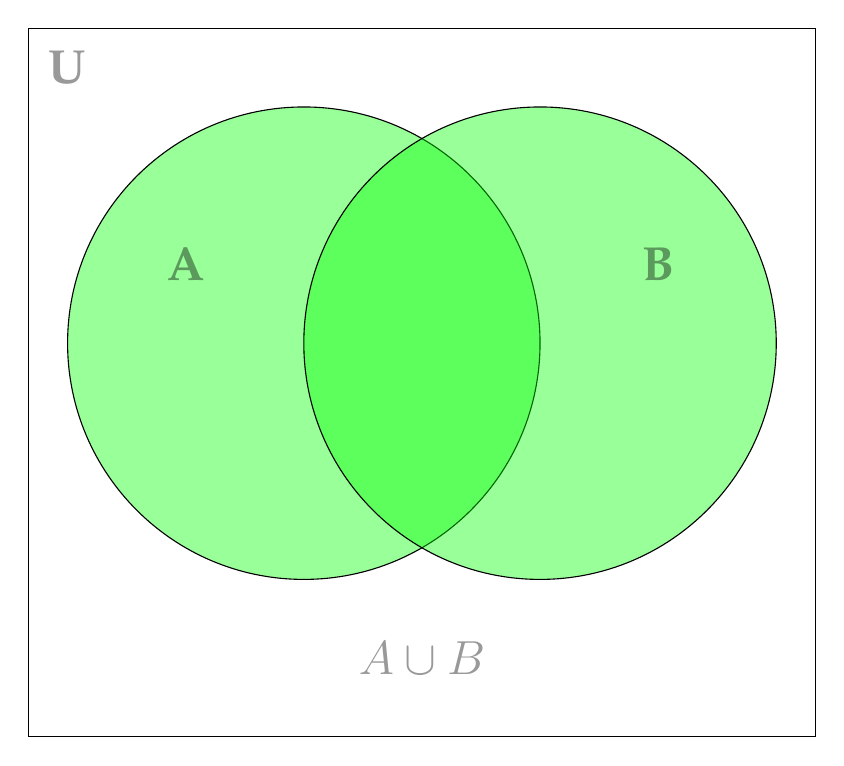
\begin{tikzpicture}
\begin{scope} [fill opacity = .4]
    \draw (-5,5) rectangle (5,-4);
    \draw[fill=green, draw = black] (-1.5,1) circle (3);
    \draw[fill=green, draw = black] (1.5,1) circle (3);
    \node at (-4.5,4.5) {\LARGE\textbf{U}};
    \node at (-3,2) {\LARGE\textbf{A}};
    \node at (3,2) {\LARGE\textbf{B}};
    \node at (0,-3) {\LARGE\textbf{$A \cup B$}};
    \end{scope}
%% And now you have a Venn diagram. Yay!
\end{tikzpicture}
\end{center}
\textbf{For example},\\ 
If $A = \{2,4,6,8\}$ and $B = \{6,8,10,12\}$ \\
then $A \cup B = \{2,4,6,8,10,12\}$\\
The Union operation satisfies the following properties : 
\begin{itemize}
    \item Commutative Law : $A \cup B$ = $B \cup A$
    \item Associative Law : $(A \cup B) \cup C$ = $A \cup (B \cup C)$
    \item Law of identity element : $A \cup \emptyset$ = $A$ 
    \item Idempotent Law : $A \cup A$ = $A$
    \item Law of U : $A \cup U$ = $U$
\end{itemize}

\subsection{Intersection of Sets : $A \cap B$}
\begin{displayquote}
\textbf{Definition : The intersection of two sets $A$ and $B$ is the set of all those elements which belong to both $A$ and $B$. To denote intersection symbolically, we write $A \cap B$ = \{ $x : x \in A$ and $B$\}.\\ 
The intersection of two sets is represented by the orange region in the Venn diagram below.}
\end{displayquote}
\begin{center}
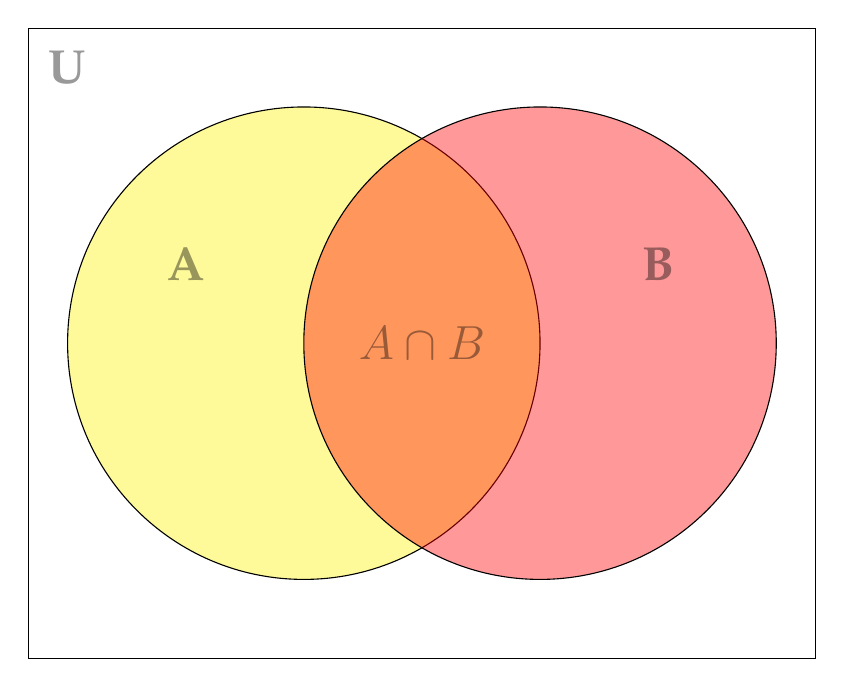
\begin{tikzpicture}
\begin{scope} [fill opacity = .4]
    \draw (-5,5) rectangle (5,-3);
    \draw[fill=yellow, draw = black] (-1.5,1) circle (3);
    \draw[fill=red, draw = black] (1.5,1) circle (3);
    \node at (-4.5,4.5) {\LARGE\textbf{U}};
    \node at (-3,2) {\LARGE\textbf{A}};
    \node at (3,2) {\LARGE\textbf{B}};
    \node at (0,1) {\LARGE\textbf{$A \cap B$}};
    \end{scope}
%% And now you have a Venn diagram. Yay!
\end{tikzpicture}
\end{center}
\textbf{For example},\\ 
If $A = \{2,4,6,8\}$ and $B = \{6,8,10,12\}$\\
then $A \cap B = \{6,8\}$\\
\textbf{Remark} : If $A$ and $B$ are two sets having no common elements such that $A \cap B$ = $\emptyset$ and thereby $n(A \cup B) = 0$, then $A$ and $B$ are called \textbf{disjoint or mutually exclusive sets}.\\
The Intersection operation satisfies the following properties : 
\begin{itemize}
    \item Commutative Law : $A \cap B$ = $B \cap A$
    \item Associative Law : $(A \cap B) \cap C$ = $A \cap (B \cap C)$
    \item Law of $\emptyset$ : $A \cap \emptyset$ = $\emptyset$
    \item Idempotent Law : $A \cap A$ = $A$
    \item Law of U : $A \cap U$ = $A$
    \item Distributive Law : $A \cap (B \cup C)$ = $(A \cap B) \cup (A \cap C)$
\end{itemize}

\subsection{Difference of Sets : $A-B$}
\begin{displayquote}
\textbf{Definition : The difference of sets $A$ and $B$ is the set of all elements which belong to $A$ but not to $B$. To denote $A$ minus $B$ Symbolically, we write $A - B$ = \{ $x : x \in A$ and $x \notin B$\}.}
\end{displayquote}

\textbf{For example},\\ 
Let $A = \{1,2,3,4,5,6\}$ and $B = \{2,4,6,8\}$.\\
Then $A-B = \{1,3,5\}$ (Since 1,3,5 belong to $A$ but not to $B$)\\
and $B-A = \{8\}$ (Since 8 belongs to $B$ but not to $A$)\\
Thus, we note that in the difference of two sets : $\mathbf{A-B \neq B-A}$.

\subsection{Complement of a Set : $A'$}
\begin{displayquote}
\textbf{ Definition : Let $U$ be the universal set and $A$ be a subset of $U$. Then the complement of $A$ is the set of all elements of $U$ which are not the elements of $A$. Symbolically we write $A'$ to denote the complement. $A' = \{ x : x \in U$ and $x \notin A$\}. \\
The complement is represented by the red region in the Venn diagram below.}
\end{displayquote}
\begin{center}
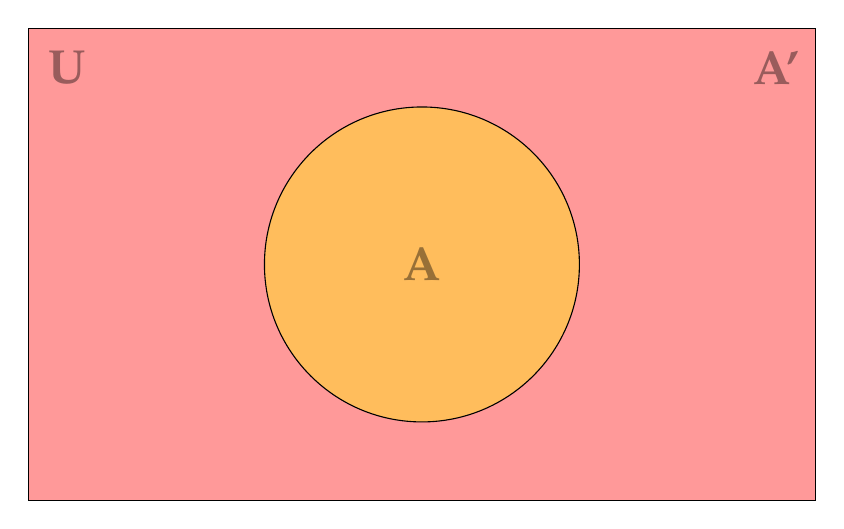
\begin{tikzpicture}
\begin{scope} [fill opacity = .4]
    \draw[fill=red] (-5,4) rectangle (5,-2);
    \draw[fill=yellow, draw = black] (0,1) circle (2);
    \node at (-4.5,3.5) {\LARGE\textbf{U}};
    \node at (4.5,3.5) {\LARGE\textbf{A'}};
    \node at (0,1) {\LARGE\textbf{A}};
    \end{scope}
%% And now you have a Venn diagram. Yay!
\end{tikzpicture}
\end{center}
As per the definition, the complement of a set $A$ can be alternatively looked upon as the difference between $U$ and $A$. Thus, It can also be denoted as : $\mathbf{A' = U-A}$.\\
\textbf{For example},\\ 
Let $U = \{1,2,3,4,5,6,7,8,9,10\}$\ and $A = \{1,3,5,7,9\}$\\
Then $A' = \{2,4,6,8,10\}$\\
The complement of a set satisfies the following properties: 
\begin{itemize}
    \item Complement Laws : $A \cup A' = U$ and $A \cap A' = \emptyset$
    \item De Morgan Laws : $(A \cup B)' = A' \cap B'$ and $(A \cap B)' = A' \cup B'$
    \item Law of double complement : $(A')' = A$
    \item Laws of empty set and universal set : $\emptyset' = U$ and $U' = \emptyset$
\end{itemize}



\section{Using Sets to Solve some Real World Problems}
In this section we will look into how sets can be used to solve practical problems. The numerical formulas derived in this section will be used extensively in the topic of probability.\\
Let $A$ and $B$ be finite sets, then :
\begin{equation}
    n(A \cup B) = n(A) + n(B) - n(A \cap B)
\end{equation}
In case, $A$ and $B$ are disjoint mutually exclusive sets, then $A \cap B = \emptyset$ and hence $n(A \cap B) = 0$. Therefore : 
\begin{equation}
    n(A \cup B) = n(A) + n(B)
\end{equation}
Now considering three sets $A$, $B$, $C$, we have : 
\begin{equation}
    n(A \cup B \cup C) = n(A) + n(B) + n(C) - n(A \cap B) - n(B \cap C) - n(A \cap C) + n(A \cap B \cap C)
\end{equation}
And in case $A$, $B$ and $C$ are disjoint sets, then : 
\begin{equation}
    n(A \cup B \cup C) = n(A) + n(B) + n(C)
\end{equation}
\begin{displayquote}
\textbf{Note : Always use Venn diagrams to help visualize when solving problems on Sets or visualizing operations on Sets and their properties.}
\end{displayquote}

\section{Solved Exercises}

\subsection{}
Show that $A \subset B$ and $B \subset A$ $\Rightarrow$ $A = B$.\\
\textbf{Solution} : \\
If $A \subset B$\\
$\Rightarrow$ $A \cap B = A$ (By Definition of Subset) \\
and If, $B \subset A$ \\
$\Rightarrow$ $A \cap B = B$ (By Definition of Subset) \\
Hence Proved : $A \cap B = A = B$.

\subsection{}
A college awarded 38 medals in football, 15 in tennis and 20 in cricket. If these medals went to a total of 58 men and only 3 men got medals in all three sports, how many received medals in exactly two of the three sports ?
\begin{center}
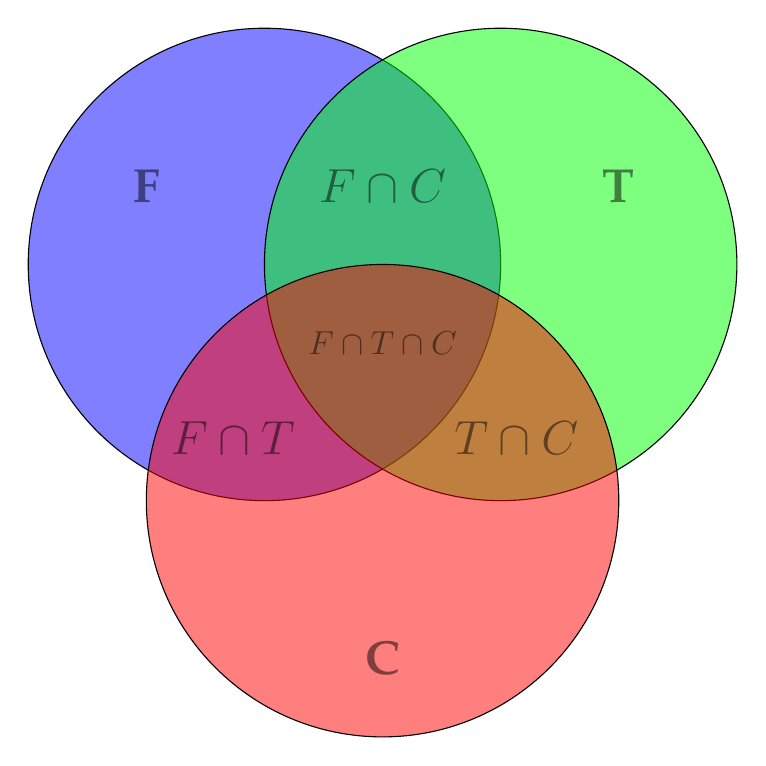
\begin{tikzpicture}
\begin{scope} [fill opacity = .5]
    %\draw (-5,5) rectangle (5,-6);
    \draw[fill=blue, draw = black] (-1.5,1) circle (3);
    \draw[fill=green, draw = black] (1.5,1) circle (3);
    \draw[fill=red, draw = black] (0,-2) circle (3);
    \node at (-3,2) {\LARGE\textbf{F}};
    \node at (3,2) {\LARGE\textbf{T}};
    \node at (0,-4) {\LARGE\textbf{C}};
    \node at (-1.9,-1.2) {\LARGE {$F \cap T$}};
    \node at (1.7,-1.2) {\LARGE {$T \cap C$}};
    \node at (0,2) {\LARGE {$F \cap C$}};
    \node at (0,0) {\large {$F \cap T \cap C$}};
    \end{scope}
%% And now you have a Venn diagram. Yay!
\end{tikzpicture}
\end{center}
\textbf{Solution} : \\
Let $F$, $T$ and $C$ be the set of men who received medals in football, tennis and cricket respectively.\\
We are given that $n(F) = 38$, $n(T) = 15$ and $n(C) = 20$, also $n(F \cup T \cup C) = 58$ and $n(F \cap T \cap C) = 3$ \\
From equation-3 above in section-9, we can calculate : \\
$\Rightarrow$ $n(F \cap T) + n(T \cap C) + n(F \cap C) = 18$ \\
$\Rightarrow$ However, as the Venn diagram above shows : all of these sets $F \cap T$, $F \cap C$ and $T \cap C$ contain the set $F \cap T \cap C$.\\ 
$\Rightarrow$ Thus to separate the number of men who got medal in \textbf{exactly} two out of three sports, we need to subtract $n(F \cap T \cap C)$ from each one of them once.\\
$\Rightarrow$ Therefore : 18 - 3(3) = 9 is the number of men who got medals in exactly two out of three sports.

\section{References}
\begin{enumerate}
    \item Class 11 - Chapter 1 : Sets.\\ 
    NCERT Mathematics Textbook, Version 2020-21.\\
    As per Indian National Curriculum Framework 2005.
\end{enumerate}

\end{document} 
